% architecture.tex — Dual-platform system architecture diagram
% Standalone TikZ figure; can also be \input{} into main.tex
% Compile: pdflatex architecture.tex
\documentclass[tikz,border=4pt]{standalone}

\usepackage{tikz}
\usetikzlibrary{arrows.meta, positioning, shapes.geometric,
                calc, fit, backgrounds}

% ── Shared colour palette ────────────────────────────────────────────────────
\definecolor{CloudBlue}    {RGB}{ 40, 110, 200}
\definecolor{CloudBg}      {RGB}{215, 232, 255}
\definecolor{ModalPurple}  {RGB}{120,  60, 185}
\definecolor{ModalBg}      {RGB}{238, 220, 255}
\definecolor{ServiceGreen} {RGB}{ 40, 155,  90}
\definecolor{ServiceBg}    {RGB}{218, 248, 228}
\definecolor{ArrowGray}    {RGB}{ 80,  85, 100}
\definecolor{PanelBg}      {RGB}{248, 250, 252}
\definecolor{PanelBorder}  {RGB}{200, 208, 218}
\definecolor{LabelGray}    {RGB}{120, 128, 140}

% ── Node styles ─────────────────────────────────────────────────────────────
\tikzset{
  % Platform header box
  platform/.style={
    rectangle, rounded corners=6pt,
    fill=#1!15, draw=#1, line width=1.2pt,
    font=\bfseries\scriptsize, text=#1,
    inner sep=7pt, minimum width=4.8cm, minimum height=0.68cm,
    align=center
  },
  platform/.default=CloudBlue,
  % Sub-component inside a platform
  subcomp/.style={
    rectangle, rounded corners=4pt,
    fill=white, draw=#1!60, line width=0.75pt,
    font=\scriptsize, text=black,
    inner sep=4pt, minimum width=2.1cm, minimum height=0.55cm,
    align=center
  },
  subcomp/.default=CloudBlue,
  % External service node
  service/.style={
    rectangle, rounded corners=5pt,
    fill=ServiceBg, draw=ServiceGreen, line width=0.9pt,
    font=\scriptsize\bfseries, text=ServiceGreen,
    inner sep=5pt, minimum width=2.1cm, minimum height=0.58cm,
    align=center
  },
  % Stat badge (small annotation)
  statbadge/.style={
    font=\tiny, text=LabelGray, align=center
  },
  % Data-flow arrows
  dataarrow/.style={
    ->, >=Stealth, line width=0.75pt, color=ArrowGray
  },
  dataarrow_blue/.style={
    ->, >=Stealth, line width=0.75pt, color=CloudBlue!80, dashed
  },
  dataarrow_purple/.style={
    ->, >=Stealth, line width=0.75pt, color=ModalPurple!80, dashed
  }
}

\begin{document}
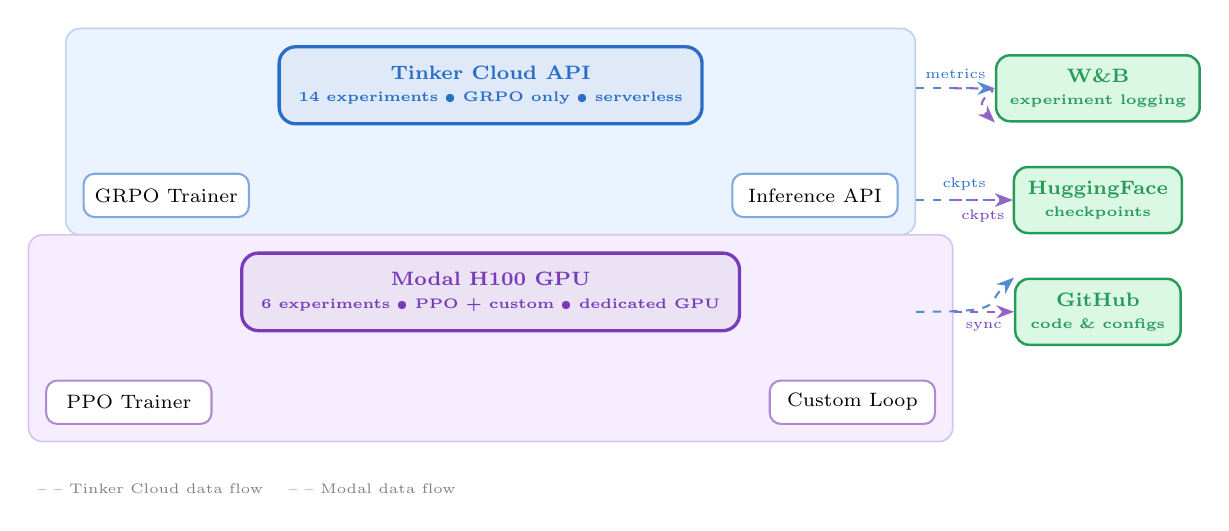
\begin{tikzpicture}[node distance=0.5cm and 0.7cm]

  % ── PLATFORM A: Tinker Cloud ──────────────────────────────────────────────
  \node[platform=CloudBlue] (cloud_hdr)
        {Tinker Cloud API\\\tiny 14 experiments \textbullet{} GRPO only \textbullet{} serverless};

  % Sub-components inside Cloud platform
  \node[subcomp=CloudBlue, below left=0.6cm and 0.35cm of cloud_hdr]  (c_grpo)
        {GRPO Trainer};
  \node[subcomp=CloudBlue, below right=0.6cm and 0.35cm of cloud_hdr] (c_inf)
        {Inference API};

  % Fit a background panel around cloud components
  \begin{scope}[on background layer]
    \node[rectangle, rounded corners=5pt,
          fill=CloudBg!50, draw=CloudBlue!30, line width=0.6pt,
          fit=(cloud_hdr)(c_grpo)(c_inf), inner sep=6pt] (cloud_panel) {};
  \end{scope}

  % ── PLATFORM B: Modal H100 ────────────────────────────────────────────────
  \node[platform=ModalPurple, below=1.6cm of cloud_hdr] (modal_hdr)
        {Modal H100 GPU\\\tiny 6 experiments \textbullet{} PPO + custom \textbullet{} dedicated GPU};

  % Sub-components inside Modal platform
  \node[subcomp=ModalPurple, below left=0.6cm and 0.35cm of modal_hdr]  (m_ppo)
        {PPO Trainer};
  \node[subcomp=ModalPurple, below right=0.6cm and 0.35cm of modal_hdr] (m_cust)
        {Custom Loop};

  % Fit a background panel around modal components
  \begin{scope}[on background layer]
    \node[rectangle, rounded corners=5pt,
          fill=ModalBg!50, draw=ModalPurple!30, line width=0.6pt,
          fit=(modal_hdr)(m_ppo)(m_cust), inner sep=6pt] (modal_panel) {};
  \end{scope}

  % ── EXTERNAL SERVICES (right column) ─────────────────────────────────────
  % Place them to the right of the platform panels
  \node[service, right=1.0cm of cloud_panel.east, yshift=0.55cm] (wb)
        {W\&B\\{\tiny experiment logging}};

  \node[service, below=0.55cm of wb] (hf)
        {HuggingFace\\{\tiny checkpoints}};

  \node[service, below=0.55cm of hf] (gh)
        {GitHub\\{\tiny code \& configs}};

  % ── ARROWS: platforms → external services ────────────────────────────────

  % Cloud → W&B
  \draw[dataarrow_blue]
        (cloud_panel.east |- wb.west) -- node[above, font=\tiny, text=CloudBlue]{metrics} (wb.west);

  % Cloud → HuggingFace
  \draw[dataarrow_blue]
        (cloud_panel.east |- hf.west) -- node[above, font=\tiny, text=CloudBlue]{ckpts} (hf.west);

  % Modal → W&B
  \draw[dataarrow_purple]
        (modal_panel.east |- wb.west)
        .. controls +(1.0,0) and +(-0.4,0.4) ..
        (wb.south west);

  % Modal → HuggingFace
  \draw[dataarrow_purple]
        (modal_panel.east |- hf.west) -- node[below, font=\tiny, text=ModalPurple]{ckpts} (hf.west);

  % Modal → GitHub
  \draw[dataarrow_purple]
        (modal_panel.east |- gh.west) -- node[below, font=\tiny, text=ModalPurple]{sync} (gh.west);

  % Cloud → GitHub
  \draw[dataarrow_blue]
        (cloud_panel.east |- gh.west)
        .. controls +(1.2,0) and +(-0.4,-0.35) ..
        (gh.north west);

  % ── LEGEND ───────────────────────────────────────────────────────────────
  \node[font=\tiny, text=LabelGray, align=left,
        below=0.4cm of modal_panel.south west, anchor=north west]
  {%
    \textcolor{CloudBlue!80}{-- --} Tinker Cloud data flow \quad
    \textcolor{ModalPurple!80}{-- --} Modal data flow%
  };

\end{tikzpicture}
\end{document}
